
\begin{frame}[fragile]{Du modèle EA au schéma relationnel normalisé}

La modélisation Entité/Association nous donne toutes les informations nécessaires
pour obtenir une schéma relationnel normalisé.

\vfill

Dans cette session:

\begin{redbullet}
  \item Application de l'agorithme de normalisation à un schéma EA
  \item Illustration avec le schéma et la base des films

\end{redbullet}


\vfill
\begin{blocgauche}
\alert{Ces diapositives correspondent au support en ligne disponible sur
le site \url{http://sql.bdpedia.fr/}}
\end{blocgauche}

\end{frame}


\begin{frame}{Reprenons le schéma de la base des films}

Supposons qu'on ait validé la modélisation suivante
\vfill

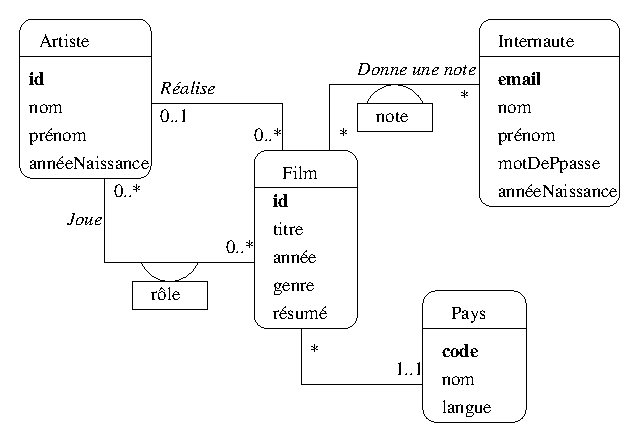
\includegraphics[width=7.5cm]{../../figures/films}

\vfill

Il n'y a plus qu'à appliquer la normalisation.
\end{frame}


%%%%%%%%%%%%
\begin{frame}{Algorithme de normalisation}


\begin{redbullet}
  \item  Chaque entité définit une DF 
    de l'identifiant vers les attributs
    $$idFilm \to titre, ann\acute{e}e, genre, r\acute{e}sum\acute{e}$$
        
  \item Chaque association plusieurs-à-un correspond à une DF 
    entre les identifiants.
    
       $$idFilm \to idArtiste$$

  \item Chaque association (binaire) plusieurs-à-plusieurs correspond à 
    une DF  entre l'identifiant
    de l'association  et ses attributs
    
    $$(idFilm, idArtiste) \to r\hat{o}le$$
\end{redbullet}


\vfill
\begin{blocgauche}
\alert{C'est tout!}
\end{blocgauche}
\end{frame}

%%%%%%%%%%%%
\begin{frame}{Résultat pour la base des films}

Clés primaires en \textbf{gras}, clés étrangères en \textit{italiques}.

\vfill
\begin{redbullet}
  \item Film (\textbf{idFilm}, titre, année, genre, résumé, \textit{idRéalisateur}, \textit{codePays})
  \item Artiste (\textbf{idArtiste}, nom, prénom, annéeNaissance)
    \item Rôle (\textbf{\textit{idFilm}, \textit{idActeur}}, nomRôle)
   \item Internaute (\textbf{email}, nom, prénom, région)
     \item Notation (\textbf{\textit{email}, \textit{idFilm}}, note)
   \item Pays (\textbf{code}, nom, langue)
\end{redbullet}


\vfill
\begin{blocgauche}
NB: le nommage des attributs est libre.
\end{blocgauche}
\end{frame}


\begin{frame}{Attention aux associations plusieurs-plusieurs sans attribut}

Une association plusieurs-plusieurs sans attribut propre
\vfill

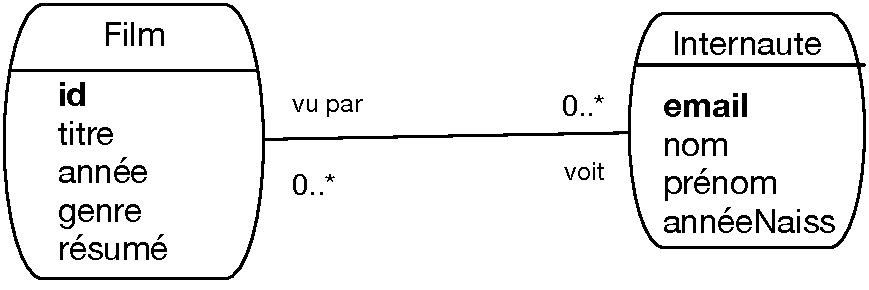
\includegraphics[width=7.5cm]{../../figures/vu-film}

\vfill
Ne pas oublier de créer la table \texttt{Vu(\textbf{idFilm, email})}
\end{frame}

%%%%%%%%%%%%
\begin{frame}{Petit exemple}


\begin{small}
\begin{center}
\begin{tabular}{l|l|c|l|c|c}
\textbf{idFilm} & titre & année  & genre & \textit{idMES} & \textit{codePays}\\
\hline
20 & Impitoyable & 1992 & Western & 100 & USA \\
21 & Ennemi d'état & 1998 & Action & 102 & USA\\
\hline
\end{tabular}

\centerline{La table \tble{Film}}
\end{center}
\begin{center}
\begin{minipage}[b]{6cm}
\begin{tabular}{l|l|l|c}
\textbf{idArtiste} &  nom & prénom &  annéeNaiss \\
\hline
100 & Eastwood & Clint  & 1930 \\
101 & Hackman & Gene  & 1930 \\
102 & Scott & Tony  & 1930 \\
103 & Smith  & Will  & 1968 \\
\hline
\end{tabular}
\centerline{La table \tble{Artiste}}
\end{minipage} \hspace*{2cm} \
\begin{minipage}[b]{5cm}
\begin{tabular}{l|c|l}
\textbf{\textit{idFilm}} & \textbf{\textit{idActeur}}  & rôle \\
\hline
20  & 100  & William Munny\\
20 & 101  & Little Bill\\
21 & 101  & Bril\\
21 & 103  & Robert Dean\\
\hline
\end{tabular}

\centerline{La table \tble{Rôle}}
\end{minipage}
\end{center}
\end{small}
\end{frame}


%%%%%%%%%%%%%
\begin{frame}{À retenir}
À partir du schéma E/A, on applique l'algorithme de normalisation et on obtient
un schéma relationnel en 3FN.

\vfill

\begin{redbullet}
   \item Pas de magie: le schéma ne sera pas meilleur que la conception
   \item Attention à ne pas ``cacher''  de dépendance fonctionnelle dans une entité
   \item On peut ajouter des contraintes, typages et contrôles quand on crée les tables
\end{redbullet}

\vfill

Cf. le support de cours pour quelques compléments (spécialisation)
\end{frame}

